\documentclass[tikz,border=2mm]{standalone}
\usepackage{tikz}
\usetikzlibrary{positioning,calc}

% ------------------------------------------------------------------
% Named colors
% ------------------------------------------------------------------
\definecolor{modelblue}{RGB}{25,101,128}
\definecolor{opgreen}{RGB}{22,109,36}
\definecolor{databrown}{RGB}{198,78,16}
\definecolor{darkoutline}{RGB}{5,34,48}

\begin{document}

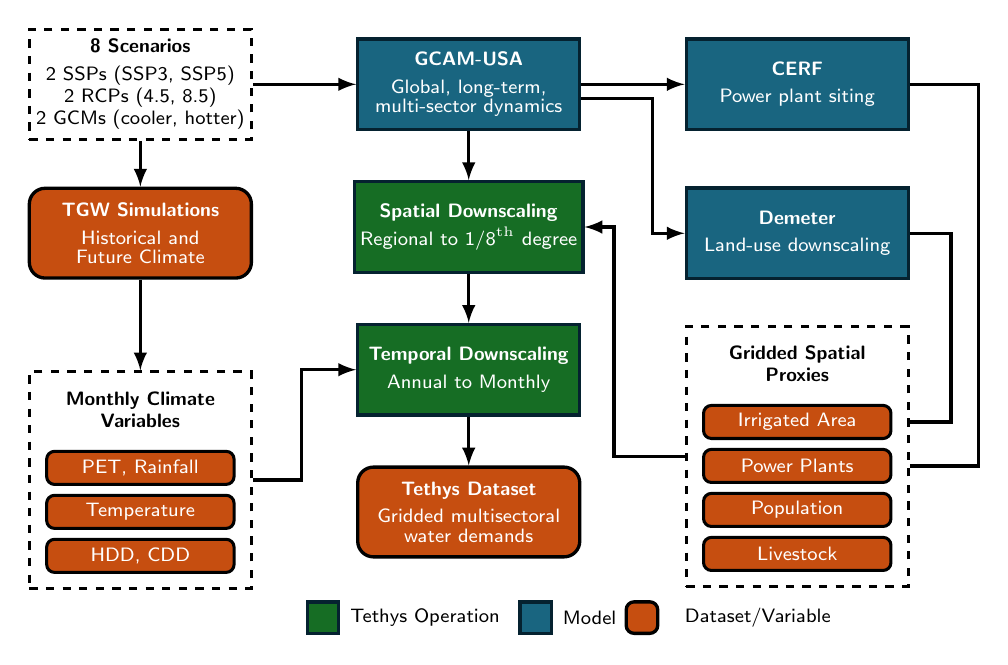
\begin{tikzpicture}[
    font=\sffamily\scriptsize,
    >=latex, % LaTeX arrow head
    arr/.style={->, line width=1.2pt, black},
    conn/.style={line width=1.2pt, black},
    dashedbox/.style={
        draw=black,
        dashed,
        line width=1.1pt,
        fill=white,
        inner sep=0pt
    },
    model/.style={
        draw=darkoutline,
        line width=1.2pt,
        fill=modelblue,
        text=white,
        minimum width=2.82cm,
        minimum height=1.15cm,
        align=center,
        inner sep=2pt
    },
    op/.style={
        draw=darkoutline,
        line width=1.2pt,
        fill=opgreen,
        text=white,
        minimum width=2.82cm,
        minimum height=1.15cm,
        align=center,
        inner sep=2pt
    },
    data/.style={
        draw=black,
        line width=1.2pt,
        fill=databrown,
        text=white,
        rounded corners=2mm,
        minimum width=2.82cm,
        minimum height=1.14cm,
        align=center,
        inner sep=2pt
    },
    smallbar/.style={
        draw=black,
        line width=1.1pt,
        fill=databrown,
        text=white,
        rounded corners=1mm,
        minimum width=2.38cm,
        minimum height=0.42cm,
        align=center,
        inner sep=1pt
    }
]

% ------------------------------------------------------------------
% Top row
% ------------------------------------------------------------------

\node[
    dashedbox,
    minimum width=2.82cm,
    minimum height=1.40cm,
    align=center
] (scen) {%
    \textbf{8 Scenarios}\\[2pt]
    2 SSPs (SSP3, SSP5)\\
    2 RCPs (4.5, 8.5)\\
    2 GCMs (cooler, hotter)
};

\node[
    model,
    right=1.31cm of scen
] (gcam) {%
    \textbf{GCAM-USA}\\[2pt]
    Global, long-term,\\[-1pt]
    multi-sector dynamics
};

\node[
    model,
    right=1.31cm of gcam
] (cerf) {%
    \textbf{CERF}\\[2pt]
    Power plant siting
};

% ------------------------------------------------------------------
% Left column
% ------------------------------------------------------------------

\node[
    data,
    below=0.58cm of scen
] (tgw) {%
    \textbf{TGW Simulations}\\[2pt]
    Historical and\\[-1pt]
    Future Climate
};

\node[
    dashedbox,
    minimum width=2.82cm,
    minimum height=2.75cm,
    below=1.15cm of tgw
] (monthly) {};

\node[
    align=center,
    font=\sffamily\scriptsize\bfseries,
    anchor=north
] (monthlytitle) at ([yshift=-0.15cm]monthly.north) {%
    Monthly Climate\\Variables
};

\node[
    smallbar,
    below=0.16cm of monthlytitle
] (pet) {PET, Rainfall};

\node[
    smallbar,
    below=0.10cm of pet
] (temp) {Temperature};

\node[
    smallbar,
    below=0.10cm of temp
] (hdd) {HDD, CDD};

% ------------------------------------------------------------------
% Center column
% ------------------------------------------------------------------

\node[
    op,
    below=0.62cm of gcam
] (spatial) {%
    \textbf{Spatial Downscaling}\\[2pt]
    Regional to 1/8$^{\mathrm{th}}$ degree
};

\node[
    op,
    below=0.62cm of spatial
] (temporal) {%
    \textbf{Temporal Downscaling}\\[2pt]
    Annual to Monthly
};

\node[
    data,
    below=0.62cm of temporal
] (tethys) {%
    \textbf{Tethys Dataset}\\[2pt]
    Gridded multisectoral\\[-1pt]
    water demands
};

% ------------------------------------------------------------------
% Right column
% ------------------------------------------------------------------

\node[
    model,
    below=0.70cm of cerf
] (demeter) {%
    \textbf{Demeter}\\[2pt]
    Land-use downscaling
};

\node[
    dashedbox,
    minimum width=2.82cm,
    minimum height=3.3cm,
    below=0.57cm of demeter
] (proxies) {};

\node[
    align=center,
    font=\sffamily\scriptsize\bfseries,
    anchor=north
] (proxiestitle) at ([yshift=-0.14cm]proxies.north) {%
    Gridded Spatial\\Proxies
};

\node[
    smallbar,
    below=0.16cm of proxiestitle
] (irr) {Irrigated Area};

\node[
    smallbar,
    below=0.10cm of irr
] (pp) {Power Plants};

\node[
    smallbar,
    below=0.10cm of pp
] (pop) {Population};

\node[
    smallbar,
    below=0.10cm of pop
] (liv) {Livestock};

% ------------------------------------------------------------------
% Arrows / connectors
% ------------------------------------------------------------------

\draw[arr] (scen.east) -- (gcam.west);
\draw[arr] (scen.south) -- (tgw.north);
\draw[arr] (tgw.south) -- (monthly.north);

\draw[arr] (gcam.south) -- (spatial.north);
\draw[arr] (spatial.south) -- (temporal.north);
\draw[arr] (temporal.south) -- (tethys.north);

\draw[arr] (gcam.east) -- (cerf.west);

\draw[arr]
    ([yshift=-0.18cm]gcam.east)
    -- ++(0.90cm,0)
    |- (demeter.west);

\draw[arr]
    (monthly.east)
    -- ++(0.62cm,0)
    |- (temporal.west);

\draw[arr]
    (proxies.west)
    -- ++(-0.90cm,0)
    |- (spatial.east);

% Right-side external connector lines
\coordinate (cerfbus) at ($(cerf.east)+(0.87cm,0)$);
\coordinate (dembus)  at ($(demeter.east)+(0.52cm,0)$);

\draw[conn]
    (cerf.east)
    -- (cerfbus)
    |- (pp.east -| proxies.east);

\draw[conn]
    (demeter.east)
    -- (dembus)
    |- (irr.east -| proxies.east);

% ------------------------------------------------------------------
% Legend
% ------------------------------------------------------------------

\coordinate (legendbase) at ($(tethys.south)+(0.75,-0.75cm)$);

\node[
    draw=darkoutline,
    line width=1.2pt,
    fill=opgreen,
    minimum width=0.40cm,
    minimum height=0.40cm
] (legopbox) at ($(legendbase)+(-2.60cm,0)$) {};

\node[
    anchor=west
] at ($(legopbox.east)+(0.00cm,0)$) {Tethys Operation};

\node[
    draw=darkoutline,
    line width=1.2pt,
    fill=modelblue,
    minimum width=0.40cm,
    minimum height=0.40cm
] (legmodelbox) at ($(legendbase)+(0.1cm,0)$) {};

\node[
    anchor=west
] at ($(legmodelbox.east)+(0.00cm,0)$) {Model};

\node[
    draw=black,
    line width=1.2pt,
    fill=databrown,
    rounded corners=1mm,
    minimum width=0.40cm,
    minimum height=0.40cm
] (legdatabox) at ($(legendbase)+(1.45cm,0)$) {};

\node[
    anchor=west
] at ($(legdatabox.east)+(0.20cm,0)$) {Dataset/Variable};

\end{tikzpicture}

\end{document}